\chapter{Introduction to Graph Theory}

\section{Introduction}

A graph consists of a nonempty set \(V\)  of vertices and a set E of edges, where each edge in \(E\) connects two (may be the same) vertices in \(V\). We usually use \(G = (V, E)\) to indicate the above relationship.

\subsection{Simple Graph}
If each edge connects two different vertices, and no two edges connect the same pair of vertices, then the graph is a simple graph. For example, the graph on the left is a simple graph, and the graph on the right is not a simple graph.

\begin{figure}[H]
  \centering
  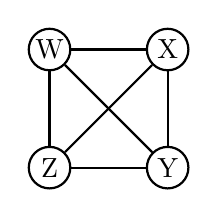
\begin{tikzpicture}[node distance={15mm}, thick, main/.style = {draw, circle}]
    \tikzstyle{vertex}=[circle,draw=black,thick,fill=white,minimum size=15pt, inner sep=0pt]
    \node[vertex] (Z) at (0, 0) {Z};
    \node[vertex] (W) at (0, 1.5) {W};
    \node[vertex] (X) at (1.5, 1.5) {X};
    \node[vertex] (Y) at (1.5, 0) {Y};
    \path
    (Z) edge (W) 
    (W) edge (X) 
    (X) edge (Y) 
    (Y) edge (Z)
    (W) edge (Y)
    (Z) edge (X)
    ;
  \end{tikzpicture}
  \quad\quad\quad
  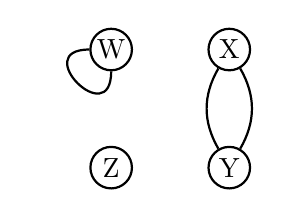
\begin{tikzpicture}[node distance={15mm}, thick, main/.style = {draw, circle}]
    \tikzstyle{vertex}=[circle,draw=black,thick,fill=white,minimum size=15pt, inner sep=0pt]
    \node[vertex] (Z) at (0, 0) {Z};
    \node[vertex] (W) at (0, 1.5) {W};
    \node[vertex] (X) at (1.5, 1.5) {X};
    \node[vertex] (Y) at (1.5, 0) {Y};
    \path
    (W) edge [out=180,in=270,looseness=5] (W)
    (X) edge [bend left] (Y)
    (X) edge [bend right] (Y)
    ;
  \end{tikzpicture}
\end{figure}

\subsection{Directed Graph}
A directed graph G consists of a nonempty set \(V\)  of vertices and a set \(E\)  of directed edges, where each edge is associated with an ordered pair of vertices. We write \(G = (V, E)\) to denote the graph. For example

\begin{figure}[H]
  \centering
  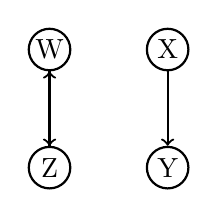
\begin{tikzpicture}[node distance={15mm}, thick, main/.style = {draw, circle}]
    \tikzstyle{vertex}=[circle,draw=black,thick,fill=white,minimum size=15pt, inner sep=0pt]
    \node[vertex] (Z) at (0, 0) {Z};
    \node[vertex] (W) at (0, 1.5) {W};
    \node[vertex] (X) at (1.5, 1.5) {X};
    \node[vertex] (Y) at (1.5, 0) {Y};
    \path[->]
    (Z) edge (W) 
    (W) edge (Z) 
    (X) edge (Y)
    ;
  \end{tikzpicture}
\end{figure}

\subsection{Undirected Graph} 
Let \(e\) be an edge that connects vertices \(u\) and \(v\). We say
\begin{itemize}
  \item \(e\) is incident with \(u\) and \(v\)
  \item \(u\) and \(v\) are the endpoints of \(e\) ;
  \item \(u\) and \(v\) are adjacent (or neighbors)
  \item if \(u\) = \(v\), the edge e is called a loop
\end{itemize}

The degree of a vertex \(v\), denoted by \(\deg(v)\), is the number of edges incident with \(v\), except that a
loop at \(v\) contributes twice to the degree of \(v\).

\begin{eg}
  Observe the following graph:
  \begin{figure}[H]
    \centering
    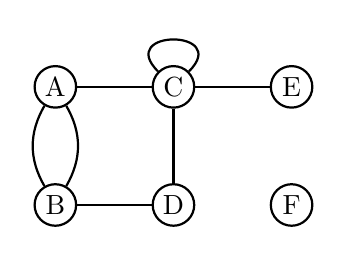
\begin{tikzpicture}[node distance={15mm}, thick, main/.style = {draw, circle}]
      \tikzstyle{vertex}=[circle,draw=black,thick,fill=white,minimum size=15pt, inner sep=0pt]
      \node[vertex] (A) at (0, 0) {A};
      \node[vertex] (B) at (0, -1.5) {B};
      \node[vertex] (C) at (1.5, 0) {C};
      \node[vertex] (D) at (1.5, -1.5) {D};
      \node[vertex] (E) at (3, 0) {E};
      \node[vertex] (F) at (3, -1.5) {F};
      \path
      (A) edge (C)
      (C) edge [out=45,in=135,looseness=5] (C)
      (C) edge (E)
      (A) edge [bend left] (B)
      (A) edge [bend right] (B)
      (B) edge (D)
      (C) edge (D)
      ;
    \end{tikzpicture}
  \end{figure}
  We have \(\deg(A) = 3,\ \deg(B) = 3,\ \deg(C) =5,\ \deg(D) = 2,\ \deg(E) = 1,\ \deg(F) = 0\)  
\end{eg}

For a simple graph \(G\) with \(n\) vertices, if it is an undirected graph, we have a maximum of \(\binom{n}{2} = \frac{n(n-1)}{2}\) edges; if it is a directed graph, then we have a maximum of \(n(n-1)\) edges. 

\begin{eg}
  Prove the proposition: among 6 people, there will be "3 mutual acquaintances" or "3 mutual strangers". Both can happen at the same time. 

  Consider a graph \(G = (V, E)\) where \(V\) is the set of people, and \(E\) indicates acquaintance. For example,
  \begin{figure}[H]
    \centering
    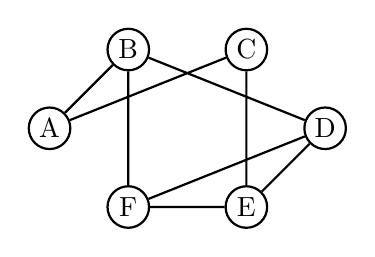
\begin{tikzpicture}[node distance={15mm}, thick, main/.style = {draw, circle}]
      \tikzstyle{vertex}=[circle,draw=black,thick,fill=white,minimum size=15pt, inner sep=0pt]
      \node[vertex] (A) at (0, 0) {A};
      \node[vertex] (B) at (1, 1) {B};
      \node[vertex] (C) at (2.5, 1) {C};
      \node[vertex] (D) at (3.5, 0) {D};
      \node[vertex] (E) at (2.5, -1) {E};
      \node[vertex] (F) at (1, -1) {F};
      \draw
      (A) -- (B)
      (A) -- (C)
      (B) -- (F)
      (B) -- (D)
      (C) -- (E)
      (F) -- (D)
      (F) -- (E)
      (E) -- (D)
      ;
    \end{tikzpicture}
  \end{figure}
  For anyone in the graph, number of neighbors + number of non-neighbors = 5.
  By pigeonhole principle, we have at least \(\lceil \frac{5}{2} \rceil = 3\) neighbor or non-neighbors for a person.  

  \textbf{Case 1}: number of neighbors of A \(\geq 3\). Let \(B, C, D\) be the neighbors, i.e. 
  \begin{figure}[H]
    \centering
    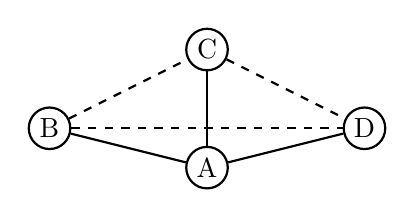
\begin{tikzpicture}[node distance={15mm}, thick, main/.style = {draw, circle}]
      \tikzstyle{vertex}=[circle,draw=black,thick,fill=white,minimum size=15pt, inner sep=0pt]
      \node[vertex] (B) at (0, 0) {B};
      \node[vertex] (C) at (2, 1) {C};
      \node[vertex] (D) at (4, 0) {D};
      \node[vertex] (A) at (2, -0.5) {A};
      \path
      (A) edge (B)
      (A) edge (C)
      (A) edge (D)
      (B) edge [dashed] (C)
      (B) edge [dashed] (D)
      (C) edge [dashed] (D)
      ;
    \end{tikzpicture}
  \end{figure}
  If \((B, C) \in E\) or \((C, D) \in E\) or \((B, D) \in E\), then we have a triangle formed by three nodes, i.e. there are three acquaintances. 

  If \((B, C) \notin E\) and \((C, D) \notin E\) and \((B, D) \notin E\), then we have three mutual strangers. 

  \textbf{Case 2}: number of non-neighbors of A \(\geq 3\). Let \(B, C, D\) be the non-neighbors, i.e. 
  \begin{figure}[H]
    \centering
    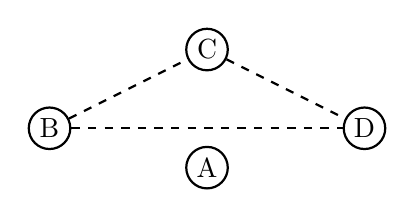
\begin{tikzpicture}[node distance={15mm}, thick, main/.style = {draw, circle}]
      \tikzstyle{vertex}=[circle,draw=black,thick,fill=white,minimum size=15pt, inner sep=0pt]
      \node[vertex] (B) at (0, 0) {B};
      \node[vertex] (C) at (2, 1) {C};
      \node[vertex] (D) at (4, 0) {D};
      \node[vertex] (A) at (2, -0.5) {A};
      \path
      (B) edge [dashed] (C)
      (B) edge [dashed] (D)
      (C) edge [dashed] (D)
      ;
    \end{tikzpicture}
  \end{figure}

  If \((B, C) \in E\) or \((C, D) \in E\) or \((B, D) \in E\), then we have a triangle formed by three nodes, i.e. there are three acquaintances. 

  Otherwise, \(A\) and at least 2 members from \(B, C, D\) will form a group of 3 mutual strangers.
\end{eg}

\subsection{Regular Graph}
A regular graph is a graph where each vertex has the same number of neighbors; i.e. every vertex has the same degree or valency. We called the graph \(k\)-regular if the common degree is \(k\).
For example, the following graph is 3-regular:
\begin{figure}[H]
  \centering
  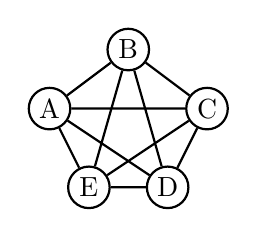
\begin{tikzpicture}[node distance={15mm}, thick, main/.style = {draw, circle}]
  \tikzstyle{vertex}=[circle,draw=black,thick,fill=white,minimum size=15pt, inner sep=0pt]
  \node[vertex] (A) at(0, 0) {A};
  \node[vertex] (B) at(1, 0.75) {B};
  \node[vertex] (C) at(2, 0) {C};
  \node[vertex] (D) at(1.5, -1) {D};
  \node[vertex] (E) at(0.5, -1) {E};
  \draw
  (A) -- (B) -- (C) -- (D) -- (E) -- (A) -- (C) -- (E) -- (B) -- (D) -- (A)
  ;
  \end{tikzpicture}
\end{figure}
If every vertex in a simple graph has the same degree, then it is also called a regular graph. However, it should be noted that a regular graph need not be a simple graph; it only needs to have the same degree for every vertex, in which loops are also allowed.

\subsection{Cartesian Product}
In graph theory, the Cartesian product \(G \times H\) of graph \(G\) and \(H\) is a graph such that:
\begin{itemize}
  \item the vertex set of \(G \times H\) is the Cartesian product \(V(G) \times V(H)\);
  \item two vertices \((u, v)\) and \((u^{\prime} , v^{\prime})\) are adjacent in \(G \times H\) if and only if either
  \begin{itemize}
    \item \(u = u^{\prime}\) and \(v\) is adjacent to \(v^{\prime}\) in \(H\) or 
    \item \(v = v^{\prime}\) and \(u\) is adjacent to \(u^{\prime}\) in \(G\)
  \end{itemize}
\end{itemize}
For example:

\begin{minipage}{.3\textwidth}
  \begin{figure}[H]
    \centering
    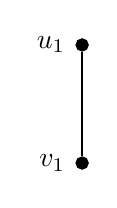
\begin{tikzpicture}[node distance={15mm}, thick, main/.style = {draw, circle}]
      \tikzstyle{vertex}=[circle,draw=black,thick,fill=black,minimum size=4pt, inner sep=0pt]
      \node[vertex][label=left:{\(u_1\)}] (u1) at(0, 0) {};
      \node[vertex][label=left:{\(v_1\)}] (v1) at(0, -1.5) {};
      \draw
      (u1) -- (v1)
      ;
      \end{tikzpicture}
      \caption*{\(G_1\)}
  \end{figure}
\end{minipage}
\begin{minipage}{.3\textwidth}
  \begin{figure}[H]
    \centering
    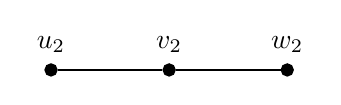
\begin{tikzpicture}[node distance={15mm}, thick, main/.style = {draw, circle}]
      \tikzstyle{vertex}=[circle,draw=black,thick,fill=black,minimum size=4pt, inner sep=0pt]
      \node[vertex][label=above:{\(u_2\)}] (u2) at(0, 0.75) {};
      \node[vertex][label=above:{\(v_2\)}] (v2) at(1.5, 0.75) {};
      \node[vertex][label=above:{\(w_2\)}] (w2) at(3, 0.75) {};
      \draw
      (u2) -- (v2) -- (w2)
      ;
      \end{tikzpicture}
      \caption*{\(G_2\)}
  \end{figure}
\end{minipage}
\begin{minipage}{.3\textwidth}
  \begin{figure}[H]
    \centering
    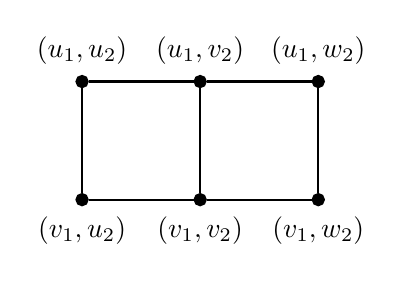
\begin{tikzpicture}[node distance={15mm}, thick, main/.style = {draw, circle}]
      \tikzstyle{vertex}=[circle,draw=black,thick,fill=black,minimum size=4pt, inner sep=0pt]
      \node[vertex][label=above:{\((u_1, u_2)\)}] (u1u2) at(0, 0) {};
      \node[vertex][label=above:{\((u_1, v_2)\)}] (u1v2) at(1.5, 0) {};
      \node[vertex][label=above:{\((u_1, w_2)\)}] (u1w2) at(3, 0) {};
      \node[vertex][label=below:{\((v_1, u_2)\)}] (v1u2) at(0, -1.5) {};
      \node[vertex][label=below:{\((v_1, v_2)\)}] (v1v2) at(1.5, -1.5) {};
      \node[vertex][label=below:{\((v_1, w_2)\)}] (v1w2) at(3, -1.5) {};
      \draw
      (u1u2) -- (u1v2) -- (u1w2) -- (v1w2) -- (v1v2) -- (v1u2) -- (u1u2)
      (u1v2) -- (v1v2)
      ;
      \end{tikzpicture}
      \caption*{\(G_1 \times G_2\)}
  \end{figure}
\end{minipage}

\subsection{Handshaking Theorem}
\begin{theorem}[Handshaking Theorem]
  Let \(G = (V, E)\) be an undirected graph with \(\vert E \vert\) edges. Since each edge \(e\) contributes exactly twice to the sum on the left side (one to each endpoint).
  \[
    \sum_{v \in V} \deg(v) = 2\vert E \vert
  \]
\end{theorem}

\begin{corollary}
  An undirected graph has an even number of vertices of odd degree.
  \[
    2\vert E \vert = \sum_{i = 1}^n \deg(v_i) = \sum_{i:\deg(v_i) = \text{odd}} \deg(v_i) + \sum_{i:\deg(v_i) = \text{even}} \deg(v_i)
  \]
  \(\sum_{i:\deg(v_i) = \text{odd}} \deg(v_i) \) is an even number, then the number of terms summed is even. Thus, the number of odd-degree vertices is even.
\end{corollary}

\newpage
\section{Simple Graph}

\begin{definition}[Simple Paths]
  A simple path in \(G\) is either a single vertex or an ordered list of distinct vertices \(v_0 - v_1 - \dots - v_k\).
\end{definition}
Consider the following graph
\begin{figure}[H]
  \centering
  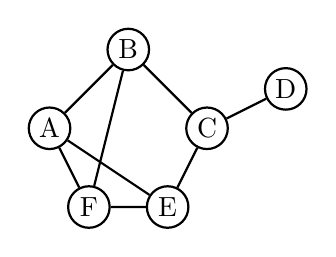
\begin{tikzpicture}[node distance={15mm}, thick, main/.style = {draw, circle}]
    \tikzstyle{vertex}=[circle,draw=black,thick,fill=white,minimum size=15pt, inner sep=0pt]
    \node[vertex] (A) at (0, 0) {A};
    \node[vertex] (B) at (1, 1) {B};
    \node[vertex] (C) at (2, 0) {C};
    \node[vertex] (D) at (3, 0.5) {D};
    \node[vertex] (E) at (1.5, -1) {E};
    \node[vertex] (F) at (0.5, -1) {F};
    \draw
    (A) -- (B) -- (C) -- (E) -- (F) -- (A)
    (A) -- (E)
    (C) -- (D)
    (B) -- (F)
    ;
  \end{tikzpicture}
\end{figure}
We then have simple path from \(C\) to \(F\): \(C - E - F\). However, \(C - B - C - E - F\) is not a simple path. 

\begin{definition}[Cycles]
  A cycle in \(G\) is a path \(v_0 - v_1 - \dots - v_k\) such that \(v_0 = v_k\) and \(k \geq 3\). 
\end{definition}
Again, by observing the graph above, we can see that one example for cycle is \(C - E - A - B - C\). However, \(C - D - C\) is not a cycle. 
The length of a path/cycle is the number of edges in the path. 

\subsection{Properties of Graphs}
\begin{itemize}
  \item A graph is connected if every pair of vertices has a path between them. (fig.1 is connected, fig.2 is not connected)
  \item A graph is acyclic if it does not contain cycle. (fig.3, fig.4)
  \item A connected, acyclic graph is called a tree. (fig.3)
  \item A leaf of a tree is a vertex of degree1. (both vertices in fig.4 are leaves)
\end{itemize}

\begin{figure}[H]
  \centering
  \begin{subfloat}[fig.1]{
  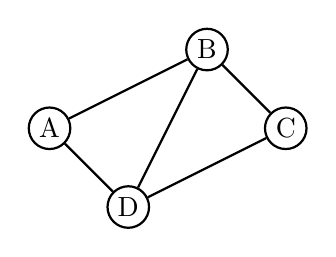
\begin{tikzpicture}[node distance={15mm}, thick, main/.style = {draw, circle}]
  \tikzstyle{vertex}=[circle,draw=black,thick,fill=white,minimum size=15pt, inner sep=0pt]
  \node[vertex] (A) at (0, 0) {A};
  \node[vertex] (B) at (2, 1) {B};
  \node[vertex] (C) at (3, 0) {C};
  \node[vertex] (D) at (1, -1) {D};
  \draw
  (A) -- (B) -- (C) -- (D) -- (A)
  (B) -- (D)
  ;
  \end{tikzpicture}
  }
  \end{subfloat}
  \hspace{10pt}
  \begin{subfloat}[fig.2]{
    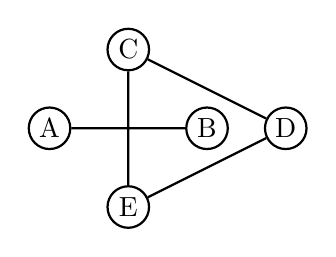
\begin{tikzpicture}[node distance={15mm}, thick, main/.style = {draw, circle}]
    \tikzstyle{vertex}=[circle,draw=black,thick,fill=white,minimum size=15pt, inner sep=0pt]
    \node[vertex] (A) at (0, 0) {A};
    \node[vertex] (B) at (2, 0) {B};
    \node[vertex] (C) at (1, 1) {C};
    \node[vertex] (D) at (3, 0) {D};
    \node[vertex] (E) at (1, -1) {E};
    \draw
    (A) -- (B)
    (C) -- (D) -- (E) -- (C)
    ;
  \end{tikzpicture}
  }
  \end{subfloat}
  \hspace{10pt}       
  \begin{subfloat}[fig.3]{
  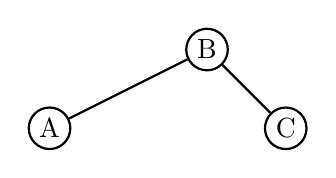
\begin{tikzpicture}[node distance={15mm}, thick, main/.style = {draw, circle}]
  \tikzstyle{vertex}=[circle,draw=black,thick,fill=white,minimum size=15pt, inner sep=0pt]
  \node[vertex] (A) at (0, 0) {A};
  \node[vertex] (B) at (2, 1) {B};
  \node[vertex] (C) at (3,0) {C};
  \draw
  (A) -- (B) -- (C)
  ;
  \end{tikzpicture}
  }
  \end{subfloat}
  \hspace{10pt}
  \begin{subfloat}[fig.4]{
  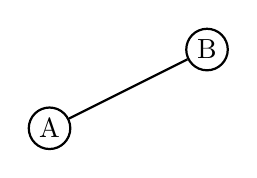
\begin{tikzpicture}[node distance={15mm}, thick, main/.style = {draw, circle}]
  \tikzstyle{vertex}=[circle,draw=black,thick,fill=white,minimum size=15pt, inner sep=0pt]
  \node[vertex] (A) at (0, 0) {A};
  \node[vertex] (B) at (2, 1) {B};
  \draw
  (A) -- (B)
  ;
  \end{tikzpicture}
  }
  \end{subfloat}
\end{figure}

\subsection{Special Simple Graphs}
A complete graph on \(n\) vertices, denoted by \(K_n\), is a simple graph that contains one edge between each pair of distinct vertices. For example, for graph \(K_5\), we have:
\begin{figure}[H]
  \centering
  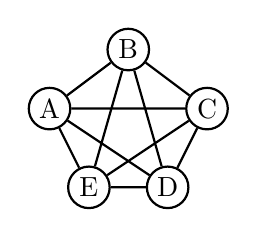
\begin{tikzpicture}[node distance={15mm}, thick, main/.style = {draw, circle}]
  \tikzstyle{vertex}=[circle,draw=black,thick,fill=white,minimum size=15pt, inner sep=0pt]
  \node[vertex] (A) at(0, 0) {A};
  \node[vertex] (B) at(1, 0.75) {B};
  \node[vertex] (C) at(2, 0) {C};
  \node[vertex] (D) at(1.5, -1) {D};
  \node[vertex] (E) at(0.5, -1) {E};
  \draw
  (A) -- (B) -- (C) -- (D) -- (E) -- (A) -- (C) -- (E) -- (B) -- (D) -- (A)
  ;
  \end{tikzpicture}
\end{figure}

An \(n\)-cube, denoted by \(Q_n\), is a graph that consists of \(2^n\)  vertices, each representing a distinct n-bit string. An edge exists between two vertices is the corresponding strings differ
in exactly one bit position.

A bipartite graph is a graph such that the vertices can be partitioned into two sets \(V\) and \(W\), so that each edge has exactly one endpoint from \(V\), and one endpoint from \(W\). 

For example, in the following graph, \(A, B, C \in V_1,\ D, E \in V_2\) such that \(V = V_1 \cup V_2,\ V_1 \cap V_2 = \varnothing\). One can also assign one of two different colors to each vertex, so that no adjacent vertices are assigned the same color. 
\begin{figure}[H]
  \centering
  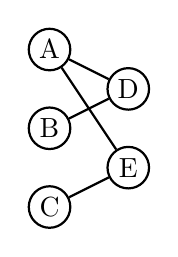
\begin{tikzpicture}[node distance={15mm}, thick, main/.style = {draw, circle}]
  \tikzstyle{vertex}=[circle,draw=black,thick,fill=white,minimum size=15pt, inner sep=0pt]
  \node[vertex] (A) at(0, 0) {A};
  \node[vertex] (B) at(0, -1) {B};
  \node[vertex] (C) at(0, -2) {C};
  \node[vertex] (D) at(1, -0.5) {D};
  \node[vertex] (E) at(1, -1.5) {E};
  \draw
  (B) -- (D) -- (A) -- (E) -- (C)
  ;
  \end{tikzpicture}
\end{figure}

\subsection{Graph Isomorphism}
A graph \(G = (V_1, E_1)\) and \(H = (V_2, E_2)\) are isomorphic if we can set up a bijection \(f: V_1 \to V_2\) such that \(x\) and \(y\) are adjacent in \(G\). For example, the following graphs are isomorphic to each other. 
\begin{figure}[H]
  \centering
  \begin{subfloat}{
  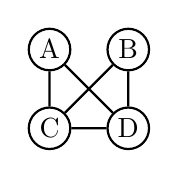
\begin{tikzpicture}[node distance={15mm}, thick, main/.style = {draw, circle}]
  \tikzstyle{vertex}=[circle,draw=black,thick,fill=white,minimum size=15pt, inner sep=0pt]
  \node[vertex] (A) at (0, 0) {A};
  \node[vertex] (B) at (1, 0) {B};
  \node[vertex] (C) at (0, -1) {C};
  \node[vertex] (D) at (1, -1) {D};
  \draw
  (D) -- (A) -- (C) -- (D) -- (B) -- (C)
  ;
  \end{tikzpicture}
  }
  \end{subfloat}
  \hspace{10pt}
  \begin{subfloat}{
    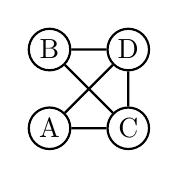
\begin{tikzpicture}[node distance={15mm}, thick, main/.style = {draw, circle}]
      \tikzstyle{vertex}=[circle,draw=black,thick,fill=white,minimum size=15pt, inner sep=0pt]
      \node[vertex] (B) at (0, 0) {B};
      \node[vertex] (D) at (1, 0) {D};
      \node[vertex] (A) at (0, -1) {A};
      \node[vertex] (C) at (1, -1) {C};
      \draw
      (D) -- (A) -- (C) -- (D) -- (B) -- (C)
      ;
      \end{tikzpicture}
  }
  \end{subfloat}
  \hspace{10pt}       
  \begin{subfloat}{
    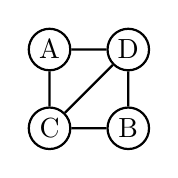
\begin{tikzpicture}[node distance={15mm}, thick, main/.style = {draw, circle}]
      \tikzstyle{vertex}=[circle,draw=black,thick,fill=white,minimum size=15pt, inner sep=0pt]
      \node[vertex] (A) at (0, 0) {A};
      \node[vertex] (D) at (1, 0) {D};
      \node[vertex] (C) at (0, -1) {C};
      \node[vertex] (B) at (1, -1) {B};
      \draw
      (D) -- (A) -- (C) -- (D) -- (B) -- (C)
      ;
      \end{tikzpicture}
  }
  \end{subfloat}
  \hspace{10pt}
  \begin{subfloat}{
    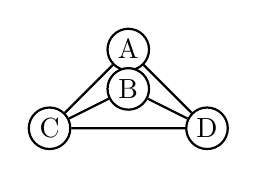
\begin{tikzpicture}[node distance={15mm}, thick, main/.style = {draw, circle}]
      \tikzstyle{vertex}=[circle,draw=black,thick,fill=white,minimum size=15pt, inner sep=0pt]
      \node[vertex] (A) at (0, 0) {A};
      \node[vertex] (B) at (0, -0.5) {B};
      \node[vertex] (C) at (-1, -1) {C};
      \node[vertex] (D) at (1, -1) {D};
      \draw
      (D) -- (A) -- (C) -- (D) -- (B) -- (C)
      ;
      \end{tikzpicture}
  }
  \end{subfloat}
\end{figure}
By observation, one can see that if two graphs are isomorphic, then the adjacent vertices in the original graph will still be adjacent, and the degree of such vertices also remains unchanged.

\section{Graph Search}
\subsection{Eulerian Paths and Circuits}
In graph theory, an Eulerian path in a graph is a path that contains each edge exactly once (allowing for revisiting vertices). If such a path is also a circuit, it is called an Eulerian circuit. For example, the following graph contains an Eulerian path:
\begin{figure}[H]
  \centering
  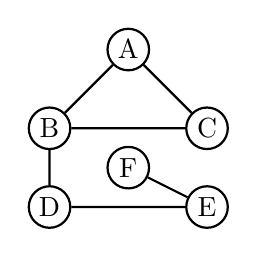
\begin{tikzpicture}[node distance={15mm}, thick, main/.style = {draw, circle}]
  \tikzstyle{vertex}=[circle,draw=black,thick,fill=white,minimum size=15pt, inner sep=0pt]
  \node[vertex] (A) at(0, 0) {A};
  \node[vertex] (B) at(-1, -1) {B};
  \node[vertex] (C) at(1, -1) {C};
  \node[vertex] (D) at(-1, -2) {D};
  \node[vertex] (E) at(1, -2) {E};
  \node[vertex] (F) at(0, -1.5) {F};
  \draw
  (B) -- (C) -- (A) -- (B) -- (D) -- (E) -- (F)
  ;
  \end{tikzpicture}
\end{figure}
\begin{remark}
  A connected graph \(G\) has an Eulerian circuit if and only if each vertex of \(G\) has even degree.
\end{remark}

\newpage
\subsection{Graph Representation}
We can use the adjacency matrix or adjacency list to represent an undirected graph.
\begin{eg}
Below shows two types of graph representation:

\begin{minipage}{.3\textwidth}
  \centering
  Undirected Graph
\begin{figure}[H]
  \centering
  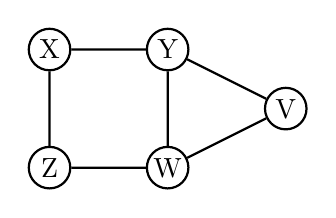
\begin{tikzpicture}[node distance={15mm}, thick, main/.style = {draw, circle}]
  \tikzstyle{vertex}=[circle,draw=black,thick,fill=white,minimum size=15pt, inner sep=0pt]
  \node[vertex] (X) at (0, 0) {X};
  \node[vertex] (Y) at (1.5, 0) {Y};
  \node[vertex] (Z) at (0, -1.5) {Z};
  \node[vertex] (W) at (1.5, -1.5) {W};
  \node[vertex] (V) at (3, -0.75) {V};
  \draw
  (Y) -- (X) -- (Z) -- (W) -- (Y) -- (V) -- (W)
  ;
  \end{tikzpicture}
\end{figure}
\end{minipage}
\begin{minipage}{.3\textwidth}
  \centering
  Adjacency Matrix
  \[
    \begin{bNiceMatrix}[first-row,first-col]
        & \text{X} & \text{Y} & \text{Z} & \text{W} & \text{V} \\
      \text{X} & 0 & 1 & 1 & 0 & 0 \\
      \text{Y} & 1 & 0 & 0 & 1 & 1 \\
      \text{Z} & 1 & 0 & 0 & 1 & 0 \\
      \text{W} & 0 & 1 & 1 & 0 & 1 \\
      \text{V} & 0 & 1 & 0 & 1 & 0 \\
  \end{bNiceMatrix}
  \]
\end{minipage}
\begin{minipage}{.3\textwidth}
  \centering
  Adjacency List
  \begin{tabular}{l l}
      [0] & X \(\to\) Y \(\to\) Z \\\relax
      [1] & Y \(\to\) X \(\to\) W \(\to\) V \\\relax
      [2] & Z \(\to\) X \(\to\) W \\\relax
      [3] & W \(\to\) Y \(\to\) Z \(\to\) V \\\relax
      [4] & V \(\to\) Y \(\to\) W \\
    \end{tabular}
\end{minipage}
\end{eg}

\subsection{Breadth-First Search (BFS)}
For Breadth-First Search, we have graph \(G = (V, E)\) as input, and source vertex \(s \in V\). Then, the distance (\(d[u]\)) from \(s\) to \(u\), for all \(u \in V\), and \(\pi [u]\), which is the predecessor of \(u\) are the outputs.
One can take the idea of Breadth-First Search as a wave spread out from one vertex.
\begin{eg}
  Consider the following graph. 
  \begin{figure}[H]
    \centering
    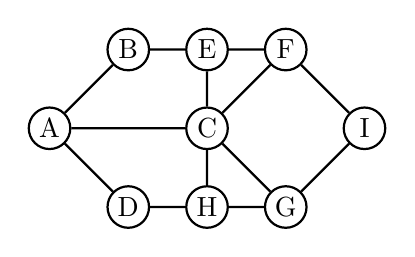
\begin{tikzpicture}[node distance={15mm}, thick, main/.style = {draw, circle}]
    \tikzstyle{vertex}=[circle,draw=black,thick,fill=white,minimum size=15pt, inner sep=0pt]
    \node[vertex] (A) at (0, 0) {A};
    \node[vertex] (B) at (1, 1) {B};
    \node[vertex] (E) at (2, 1) {E};
    \node[vertex] (F) at (3, 1) {F};
    \node[vertex] (I) at (4, 0) {I};
    \node[vertex] (C) at (2, 0) {C};
    \node[vertex] (D) at (1, -1) {D};
    \node[vertex] (H) at (2, -1) {H};
    \node[vertex] (G) at (3, -1) {G};
    \draw
    (A) -- (B) -- (E) -- (F) -- (I) -- (G) -- (H) -- (D) -- (A) -- (C) -- (F)
    (C) -- (G)
    (E) -- (C) -- (H)
    ;
    \end{tikzpicture}
  \end{figure}
    We have the following traversal:
    A \(\to\) B \(\to\) C \(\to\) D \(\to\) E \(\to\) F \(\to\) H \(\to\) I \(\to\) G. 

    We can also use the following adjacency list to show the same result
    \begin{table}[H]
      \centering
      \begin{tabular}{l|l}
          Node & Queue  \\
        \midrule
          A & (1, B), (1, C), (1, D) \\
          B & (1, C), (1, D), (1, E) \\
          C & (1, D), (1, E), (1, F), (1, G), (1, H) \\
          D & (1, E), (1, F), (1, G), (1, H) \\
          E & (1, F), (1, G), (1, H) \\
          F & (1, G), (1, H), (1, I) \\
          G & (1, H), (1, I) \\
          H & (1, I) \\
          I & -
      \end{tabular}
    \end{table}
  Then, for predecessor and distance, we have:
  \begin{table}[H]
    \centering
    \begin{tabular}{c|c|c|c|c|c|c|c|c|c}
      \(u\)  & A & B & C & D & E & F & G & H & I  \\
      \midrule
      \(\pi[u]\) &   & A & A & A & B & C & C & C & F \\
      \midrule
      \(d[u]\) & 0 & 1 & 1 & 1 & 2 & 2 & 2 & 2 & 3 \\
    \end{tabular}
  \end{table}
\end{eg}

\newpage
\subsection{Depth-First Search (DFS)}
For Depth-First Search, we have graph \(G = (V, E)\) as input, and source vertex \(s \in V\). Then, the discovery time (\(d[v]\)) from \(s\) to \(v\), for all \(v \in V\), and \(f[v]\), which is the finishing time are the outputs.
Depth-First Search is just like when we discover a vertex, we explore from it as far as we can. 
\begin{eg}
  Consider the following graph.
  \begin{figure}[H]
    \centering
    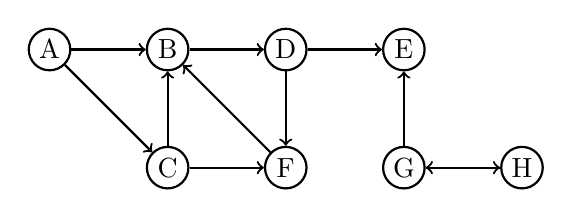
\begin{tikzpicture}[node distance={15mm}, thick, main/.style = {draw, circle}]
    \tikzstyle{vertex}=[circle,draw=black,thick,fill=white,minimum size=15pt, inner sep=0pt]
    \node[vertex] (A) at (0, 0) {A};
    \node[vertex] (B) at (1.5, 0) {B};
    \node[vertex] (D) at (3, 0) {D};
    \node[vertex] (E) at (4.5, 0) {E};
    \node[vertex] (C) at (1.5, -1.5) {C};
    \node[vertex] (F) at (3, -1.5) {F};
    \node[vertex] (G) at (4.5, -1.5) {G};
    \node[vertex] (H) at (6, -1.5) {H};
    \path[->]
    (A) edge (B)
    (B) edge (D)
    (D) edge (E)
    (A) edge (C)
    (C) edge (F)
    (F) edge (B)
    (C) edge (B)
    (D) edge (F)
    (G) edge (H)
    (H) edge (G)
    (G) edge (E)
    ;
    \end{tikzpicture}
  \end{figure}
  By using Depth-First Search, we have the following traversal:
  \begin{figure}[H]
    \centering
    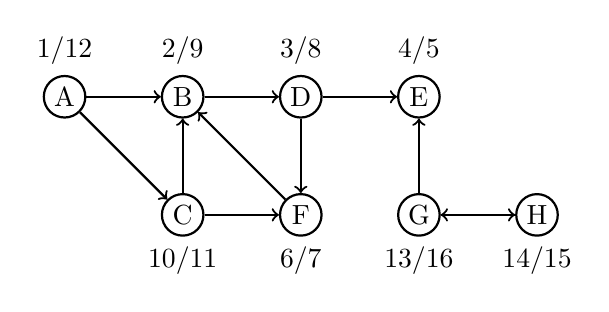
\begin{tikzpicture}[node distance={15mm}, thick, main/.style = {draw, circle}]
    \tikzstyle{vertex}=[circle,draw=black,thick,fill=white,minimum size=15pt, inner sep=0pt]
    \node[vertex][label={1/12}] (A) at (0, 0) {A};
    \node[vertex][label={2/9}] (B) at (1.5, 0) {B};
    \node[vertex][label={3/8}] (D) at (3, 0) {D};
    \node[vertex][label={4/5}] (E) at (4.5, 0) {E};
    \node[vertex][label=below:{10/11}] (C) at (1.5, -1.5) {C};
    \node[vertex][label=below:{6/7}] (F) at (3, -1.5) {F};
    \node[vertex][label=below:{13/16}] (G) at (4.5, -1.5) {G};
    \node[vertex][label=below:{14/15}] (H) at (6, -1.5) {H};
    \path[->]
    (A) edge (B)
    (B) edge (D)
    (D) edge (E)
    (A) edge (C)
    (C) edge (F)
    (F) edge (B)
    (C) edge (B)
    (D) edge (F)
    (G) edge (H)
    (H) edge (G)
    (G) edge (E)
    ;
    \end{tikzpicture}
  \end{figure}
  We use the notation "\(d[v]/f[v]\)" to show the discovery and finishing time. For example, the discovery time of node A is 1, finishing time is 12, then we use "1/12" to denote this timestamp.
  For discovery time and finishing time, we also have:
  \begin{table}[H]
    \centering
    \begin{tabular}{c|c|c|c|c|c|c|c|c|c}
      \(v\)  & A & B & C & D & E & F & G & H \\
      \midrule
      \(d[v]\) & 1 & 2 & 10 & 3 & 4 & 6 & 13 & 14 \\
      \midrule
      \(f[v]\) & 12 & 9 & 11 & 8 & 5 & 7 & 16 & 15 \\
    \end{tabular}
  \end{table}
\end{eg}

A graph is said to be strongly connected if every vertex is reachable from every other vertex. The strongly connected components of an arbitrary directed graph form a partition into subgraphs that are themselves strongly connected.

A vertex \(v\) is an articulation point (also called articulation vertex) if removing \(v\) increases the number of connected components.

A topological sort or topological ordering of a directed graph is a linear ordering of its vertices such that for every directed edge \(uv\) from vertex \(u\) to vertex \(v\), \(u\) comes before \(v\) in the ordering. Topological sorting can only be used on directed acyclic graphs. If a graph contains cycles, it cannot be topologically sorted.

\begin{eg}[Topological Sort]
  Consider the following graph.
  \begin{figure}[H]
    \centering
    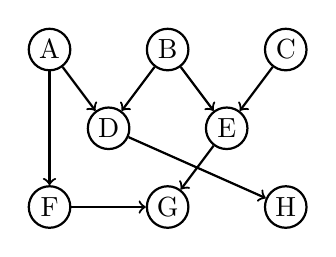
\begin{tikzpicture}[node distance={15mm}, thick, main/.style = {draw, circle}]
    \tikzstyle{vertex}=[circle,draw=black,thick,fill=white,minimum size=15pt, inner sep=0pt]
    \node[vertex] (A) at (0, 0) {A};
    \node[vertex] (B) at (1.5, 0) {B};
    \node[vertex] (C) at (3, 0) {C};
    \node[vertex] (D) at (0.75, -1) {D};
    \node[vertex] (E) at (2.25, -1) {E};
    \node[vertex] (F) at (0, -2) {F};
    \node[vertex] (G) at (1.5, -2) {G};
    \node[vertex] (H) at (3, -2) {H};
    \path[->]
    (A) edge (D)
    (A) edge (F)
    (B) edge (D)
    (B) edge (E)
    (C) edge (E)
    (E) edge (G)
    (F) edge (G)
    (D) edge (H)
    ;
    \end{tikzpicture}
  \end{figure}
  \newpage
  We can use DFS to find the topological order. We first select an unvisited node; for example, we choose node \textbf{B} in this case.
  \begin{figure}[H]
    \centering
    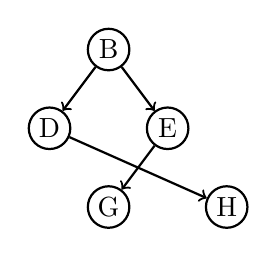
\begin{tikzpicture}[node distance={15mm}, thick, main/.style = {draw, circle}]
    \tikzstyle{vertex}=[circle,draw=black,thick,fill=white,minimum size=15pt, inner sep=0pt]
    \node[vertex] (B) at (1.5, 0) {B};
    \node[vertex] (D) at (0.75, -1) {D};
    \node[vertex] (E) at (2.25, -1) {E};
    \node[vertex] (G) at (1.5, -2) {G};
    \node[vertex] (H) at (3, -2) {H};
    \path[->]
    (B) edge (D)
    (B) edge (E)
    (E) edge (G)
    (D) edge (H)
    ;
    \end{tikzpicture}
  \end{figure}
  We have: B \(\to\) D \(\to\) E \(\to\) H \(\to\) G
  Then, we choose another node, in this case we choose node \textbf{A}.
  \begin{figure}[H]
    \centering
    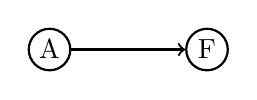
\begin{tikzpicture}[node distance={15mm}, thick, main/.style = {draw, circle}]
    \tikzstyle{vertex}=[circle,draw=black,thick,fill=white,minimum size=15pt, inner sep=0pt]
    \node[vertex] (A) at (0, 0) {A};
    \node[vertex] (F) at (2, 0) {F};
    \path[->]
    (A) edge (F)
    ;
    \end{tikzpicture}
  \end{figure}
  We have: A \(\to\) F \(\to\) B \(\to\) D \(\to\) E \(\to\) H \(\to\) G. 

  Finally, we have C \(\to\) A \(\to\) F \(\to\) B \(\to\) D \(\to\) E \(\to\) H \(\to\) G.

  This is one of the possible topological sorts. 
\end{eg}

\subsection{Shortest Path Problem}
Consider a weighted graph, which has weighted edges. We define such a graph by \(G = (V, E, w)\), where the newly introduced parameter \(w\) is the weight of an edge. Then how do we find the shortest path on a large graph from one point to another? We can use Dijkstra's Algorithm. 

We initialize the algorithm by (A) maintain a table of cost \(c(v)\), where starting vertex has cost \(c(v_0) = 0\), and other vertices have cost \(c(v_i) = \infty, i \neq 0\); (B) maintain a set of visited vertices \(S = \varnothing\). After choosing the unvisited vertex with minimum cost, we update the cost of its adjacent vertices. After updating, we repeat this process. When every vertex is visited, the algorithm will then end. These operations are called relaxation.

\begin{eg}[Shortest Path Problem]
  Consider the following graph, find the shortest path from vertex \textit{A} to vertex \textit{Z}.
  \begin{figure}[H]
  \centering
  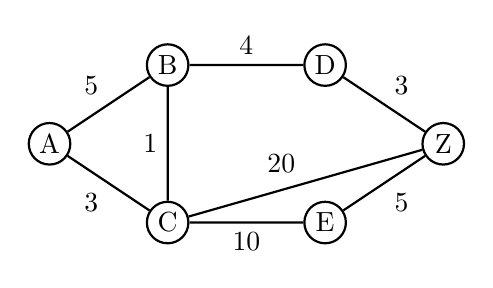
\begin{tikzpicture}[node distance={15mm}, thick, main/.style = {draw, circle}]
    \tikzstyle{vertex}=[circle,draw=black,thick,fill=white,minimum size=15pt, inner sep=0pt]
    \node[vertex] (A) at (0, 0) {A};
    \node[vertex] (B) at (1.5, 1) {B};
    \node[vertex] (C) at (1.5, -1) {C};
    \node[vertex] (D) at (3.5, 1) {D};
    \node[vertex] (E) at (3.5, -1) {E};
    \node[vertex] (Z) at (5, 0) {Z};
    \draw
    (A) -- node[anchor=south east]{5} (B)
    (B) -- node[above]{4} (D)
    (D) -- node[anchor=south west]{3} (Z)
    (Z) -- node[anchor=north west]{5} (E)
    (E) -- node[below]{10} (C)
    (C) -- node[anchor=north east]{3} (A)
    (B) -- node[left]{1} (C)
    (C) -- node[anchor=south east]{20} (Z)
    ;
  \end{tikzpicture}
\end{figure}
To solve this problem, we can use the method mentioned above:

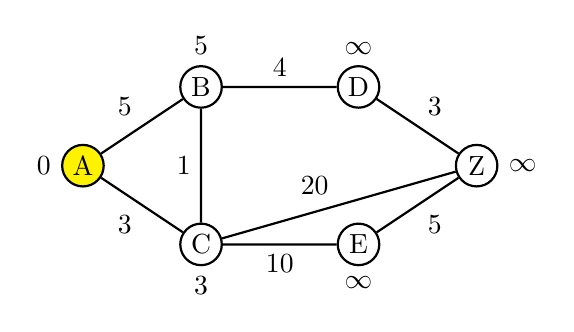
\begin{tikzpicture}[node distance={15mm}, thick, main/.style = {draw, circle}]
    \tikzstyle{vertex}=[circle,draw=black,thick,fill=white,minimum size=15pt, inner sep=0pt]
    \node[vertex,fill=yellow][label=left:{0}] (A) at (0, 0) {A};
    \node[vertex][label={5}] (B) at (1.5, 1) {B};
    \node[vertex][label=below:{3}] (C) at (1.5, -1) {C};
    \node[vertex][label={\(\infty\)}] (D) at (3.5, 1) {D};
    \node[vertex][label=below:{\(\infty\)}] (E) at (3.5, -1) {E};
    \node[vertex][label=right:{\(\infty\)}] (Z) at (5, 0) {Z};
    \draw
    (A) -- node[anchor=south east]{5} (B)
    (B) -- node[above]{4} (D)
    (D) -- node[anchor=south west]{3} (Z)
    (Z) -- node[anchor=north west]{5} (E)
    (E) -- node[below]{10} (C)
    (C) -- node[anchor=north east]{3} (A)
    (B) -- node[left]{1} (C)
    (C) -- node[anchor=south east]{20} (Z)
    ;
  \end{tikzpicture}
  \quad\quad
  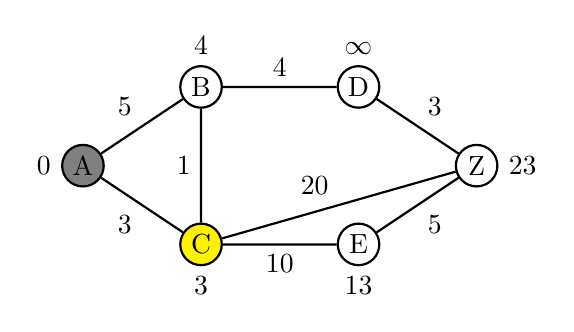
\begin{tikzpicture}[node distance={15mm}, thick, main/.style = {draw, circle}]
    \tikzstyle{vertex}=[circle,draw=black,thick,fill=white,minimum size=15pt, inner sep=0pt]
    \node[vertex,fill=gray][label=left:{0}] (A) at (0, 0) {A};
    \node[vertex][label={4}] (B) at (1.5, 1) {B};
    \node[vertex,fill=yellow][label=below:{3}] (C) at (1.5, -1) {C};
    \node[vertex][label={\(\infty\)}] (D) at (3.5, 1) {D};
    \node[vertex][label=below:{13}] (E) at (3.5, -1) {E};
    \node[vertex][label=right:{23}] (Z) at (5, 0) {Z};
    \draw
    (A) -- node[anchor=south east]{5} (B)
    (B) -- node[above]{4} (D)
    (D) -- node[anchor=south west]{3} (Z)
    (Z) -- node[anchor=north west]{5} (E)
    (E) -- node[below]{10} (C)
    (C) -- node[anchor=north east]{3} (A)
    (B) -- node[left]{1} (C)
    (C) -- node[anchor=south east]{20} (Z)
    ;
  \end{tikzpicture}

  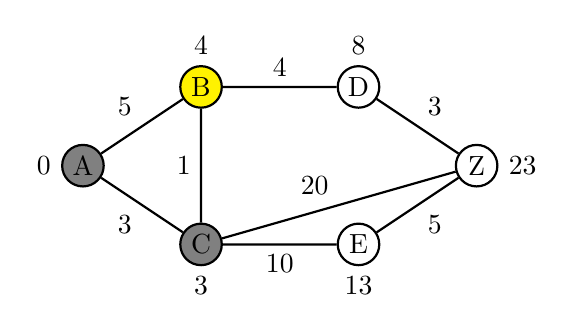
\begin{tikzpicture}[node distance={15mm}, thick, main/.style = {draw, circle}]
    \tikzstyle{vertex}=[circle,draw=black,thick,fill=white,minimum size=15pt, inner sep=0pt]
    \node[vertex,fill=gray][label=left:{0}] (A) at (0, 0) {A};
    \node[vertex,fill=yellow][label={4}] (B) at (1.5, 1) {B};
    \node[vertex,fill=gray][label=below:{3}] (C) at (1.5, -1) {C};
    \node[vertex][label={8}] (D) at (3.5, 1) {D};
    \node[vertex][label=below:{13}] (E) at (3.5, -1) {E};
    \node[vertex][label=right:{23}] (Z) at (5, 0) {Z};
    \draw
    (A) -- node[anchor=south east]{5} (B)
    (B) -- node[above]{4} (D)
    (D) -- node[anchor=south west]{3} (Z)
    (Z) -- node[anchor=north west]{5} (E)
    (E) -- node[below]{10} (C)
    (C) -- node[anchor=north east]{3} (A)
    (B) -- node[left]{1} (C)
    (C) -- node[anchor=south east]{20} (Z)
    ;
  \end{tikzpicture}
  \quad\quad
  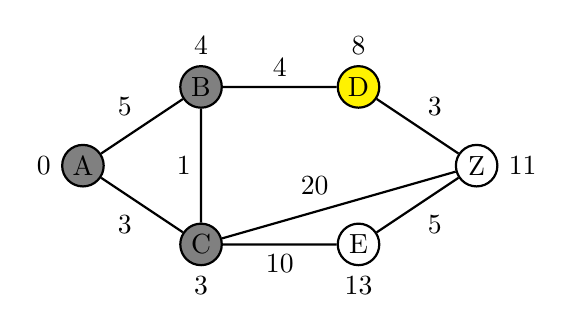
\begin{tikzpicture}[node distance={15mm}, thick, main/.style = {draw, circle}]
    \tikzstyle{vertex}=[circle,draw=black,thick,fill=white,minimum size=15pt, inner sep=0pt]
    \node[vertex,fill=gray][label=left:{0}] (A) at (0, 0) {A};
    \node[vertex,fill=gray][label={4}] (B) at (1.5, 1) {B};
    \node[vertex,fill=gray][label=below:{3}] (C) at (1.5, -1) {C};
    \node[vertex,fill=yellow][label={8}] (D) at (3.5, 1) {D};
    \node[vertex][label=below:{13}] (E) at (3.5, -1) {E};
    \node[vertex][label=right:{11}] (Z) at (5, 0) {Z};
    \draw
    (A) -- node[anchor=south east]{5} (B)
    (B) -- node[above]{4} (D)
    (D) -- node[anchor=south west]{3} (Z)
    (Z) -- node[anchor=north west]{5} (E)
    (E) -- node[below]{10} (C)
    (C) -- node[anchor=north east]{3} (A)
    (B) -- node[left]{1} (C)
    (C) -- node[anchor=south east]{20} (Z)
    ;
  \end{tikzpicture}

  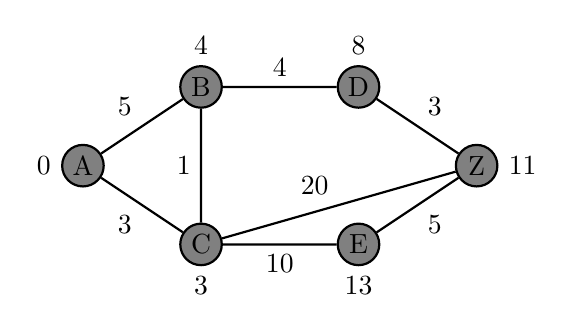
\begin{tikzpicture}[node distance={15mm}, thick, main/.style = {draw, circle}]
    \tikzstyle{vertex}=[circle,draw=black,thick,fill=white,minimum size=15pt, inner sep=0pt]
    \node[vertex,fill=gray][label=left:{0}] (A) at (0, 0) {A};
    \node[vertex,fill=gray][label={4}] (B) at (1.5, 1) {B};
    \node[vertex,fill=gray][label=below:{3}] (C) at (1.5, -1) {C};
    \node[vertex,fill=gray][label={8}] (D) at (3.5, 1) {D};
    \node[vertex,fill=gray][label=below:{13}] (E) at (3.5, -1) {E};
    \node[vertex,fill=gray][label=right:{11}] (Z) at (5, 0) {Z};
    \draw
    (A) -- node[anchor=south east]{5} (B)
    (B) -- node[above]{4} (D)
    (D) -- node[anchor=south west]{3} (Z)
    (Z) -- node[anchor=north west]{5} (E)
    (E) -- node[below]{10} (C)
    (C) -- node[anchor=north east]{3} (A)
    (B) -- node[left]{1} (C)
    (C) -- node[anchor=south east]{20} (Z)
    ;
  \end{tikzpicture}

  We can also use tables to represent the algorithm:

  \begin{minipage}{.3\textwidth}
  \begin{table}[H]
    \centering
    \begin{tabular}{c|c|c}
        \toprule
         & \(c(\cdot)\) & Path \\
      \midrule
      \colorbox{Yellow}{A} & 0 & A  \\
        B & \(\infty\) &   \\
        C & \(\infty\) &   \\
        D & \(\infty\) &   \\
        E & \(\infty\) &   \\
        Z & \(\infty\) &   \\
    \end{tabular}
    \caption*{\(S = \varnothing\)}
  \end{table}
\end{minipage}
\begin{minipage}{.3\textwidth}
  \begin{table}[H]
    \centering
    \begin{tabular}{c|c|c}
        \toprule
         & \(c(\cdot)\) & Path \\
      \midrule
      \colorbox{Gray}{A} & 0 & A  \\
        B & 5 & A, B  \\
        \colorbox{Yellow}{C} & 3 & A, C  \\
        D & \(\infty\) &   \\
        E & \(\infty\) &   \\
        Z & \(\infty\) &   \\
    \end{tabular}
    \caption*{\(S = A\)}
  \end{table}
\end{minipage}
\begin{minipage}{.3\textwidth}
  \begin{table}[H]
    \centering
    \begin{tabular}{c|c|c}
        \toprule
         & \(c(\cdot)\) & Path \\
      \midrule
      \colorbox{gray}{A} & 0 & A  \\
      \colorbox{Yellow}{B} & 4 & A, C, B  \\
      \colorbox{gray}{C} & 3 & A, C  \\
        D & \(\infty\) &   \\
        E & 13 & A, C, E  \\
        Z & 23 & A, C, Z  \\
    \end{tabular}
    \caption*{\(S = A, C\)}
  \end{table}
\end{minipage}

\begin{minipage}{.3\textwidth}
  \begin{table}[H]
    \centering
    \begin{tabular}{c|c|c}
      \toprule
       & \(c(\cdot)\) & Path \\
    \midrule
    \colorbox{Gray}{A} & 0 & A  \\
    \colorbox{Gray}{B} & 4 & A, C, B  \\
    \colorbox{Gray}{C} & 3 & A, C  \\
    \colorbox{Yellow}{D} & 8 & A, C, B, D  \\
      E & 13 & A, C, E  \\
      Z & 23 & A, C, Z  \\
  \end{tabular}
    \caption*{\(S = A, C\)}
  \end{table}
\end{minipage}
\begin{minipage}{.3\textwidth}
  \begin{table}[H]
    \centering
    \begin{tabular}{c|c|c}
      \toprule
       & \(c(\cdot)\) & Path \\
    \midrule
    \colorbox{Gray}{A} & 0 & A  \\
    \colorbox{Gray}{B} & 4 & A, C, B  \\
    \colorbox{Gray}{C} & 3 & A, C  \\
    \colorbox{Gray}{D} & 8 & A, C, B, D  \\
      E & 13 & A, C, E  \\
    \colorbox{Yellow}{Z} & 11 & A, C, B, D, Z  \\
  \end{tabular}
    \caption*{\(S = A, C, B, D\)}
  \end{table}
\end{minipage}
\begin{minipage}{.3\textwidth}
  \begin{table}[H]
    \centering
    \begin{tabular}{c|c|c}
      \toprule
       & \(c(\cdot)\) & Path \\
    \midrule
    \colorbox{Gray}{A} & 0 & A  \\
    \colorbox{Gray}{B} & 4 & A, C, B  \\
    \colorbox{Gray}{C} & 3 & A, C  \\
    \colorbox{Gray}{D} & 8 & A, C, B, D  \\
    \colorbox{Yellow}{E} & 13 & A, C, E  \\
    \colorbox{Gray}{Z} & 11 & A, C, B, D, Z  \\
  \end{tabular}
    \caption*{\(S = A, C, B, D, Z\)}
  \end{table}
\end{minipage}

Therefore, the shortest path from \(A\) to \(Z\) is \(A \to C \to B \to D \to Z\) 
\end{eg}

\subsection{Minimum Spanning Trees (MST)}
Given an undirected graph \(G = (V, E)\) with weights on the edges, a minimum spanning tree (MST) of \(G\) is an acyclic subset \(T \subseteq E\) that connects all nodes in \(V\) and whose total weight \(w(T) = \sum_{(u, v) \in T} w(u, v)\) is minimum. 

A minimum spanning tree has precisely \(n-1\) edges, where \(n\) is the number of vertices in the graph.

We have two algorithms for finding the MST. Prim's algorithm starts from finding the minimum edges among all edges, then finds the minimum edges that are connected to the vertices that are adjacent in the previous edges selected.

Kruskal's algorithm again starts from finding the minimum edges among all edges. However, we will keep finding the minimum edges until all vertices are being visited. 

\begin{eg}
  Find the minimum spanning tree for the following graph. 
  \begin{figure}[H]
    \centering
    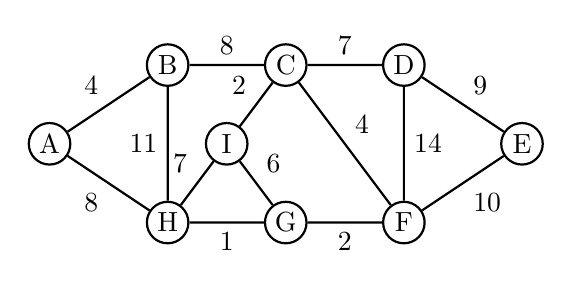
\begin{tikzpicture}[node distance={15mm}, thick, main/.style = {draw, circle}]
      \tikzstyle{vertex}=[circle,draw=black,thick,fill=white,minimum size=15pt, inner sep=0pt]
      \node[vertex] (A) at (0, 0) {A};
      \node[vertex] (B) at (1.5, 1) {B};
      \node[vertex] (C) at (3, 1) {C};
      \node[vertex] (D) at (4.5, 1) {D};
      \node[vertex] (E) at (6, 0) {E};
      \node[vertex] (F) at (4.5, -1) {F};
      \node[vertex] (G) at (3, -1) {G};
      \node[vertex] (H) at (1.5, -1) {H};
      \node[vertex] (I) at (2.25, 0) {I};
      \draw
      (A) -- node[anchor=south east]{4} (B)
      (B) -- node[above]{8} (C)
      (C) -- node[above]{7} (D)
      (D) -- node[anchor=south west]{9} (E)
      (E) -- node[anchor=north west]{10} (F)
      (F) -- node[below]{2} (G)
      (G) -- node[below]{1} (H)
      (A) -- node[anchor=north east]{8} (H)
      (B) -- node[left]{11} (H)
      (D) -- node[right]{14} (F)
      (H) -- node[anchor=south east]{7} (I)
      (I) -- node[anchor=south east]{2} (C)
      (C) -- node[anchor=south west]{4} (F)
      (I) -- node[anchor=south west]{6} (G)
      ;
    \end{tikzpicture}
  \end{figure}
\textbf{Prim's Algorithm}

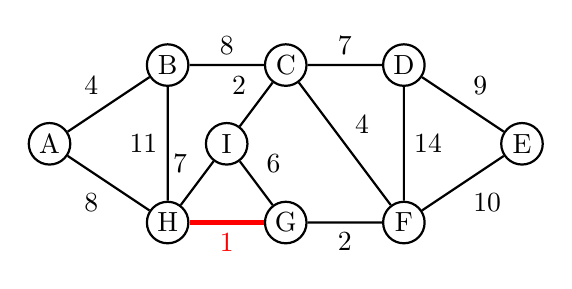
\begin{tikzpicture}[node distance={15mm}, thick, main/.style = {draw, circle}]
  \tikzstyle{vertex}=[circle,draw=black,thick,fill=white,minimum size=15pt, inner sep=0pt]
  \node[vertex] (A) at (0, 0) {A};
  \node[vertex] (B) at (1.5, 1) {B};
  \node[vertex] (C) at (3, 1) {C};
  \node[vertex] (D) at (4.5, 1) {D};
  \node[vertex] (E) at (6, 0) {E};
  \node[vertex] (F) at (4.5, -1) {F};
  \node[vertex] (G) at (3, -1) {G};
  \node[vertex] (H) at (1.5, -1) {H};
  \node[vertex] (I) at (2.25, 0) {I};
  \draw
  (A) -- node[anchor=south east]{4} (B)
  (B) -- node[above]{8} (C)
  (C) -- node[above]{7} (D)
  (D) -- node[anchor=south west]{9} (E)
  (E) -- node[anchor=north west]{10} (F)
  (F) -- node[below]{2} (G)
  (A) -- node[anchor=north east]{8} (H)
  (B) -- node[left]{11} (H)
  (D) -- node[right]{14} (F)
  (H) -- node[anchor=south east]{7} (I)
  (C) -- node[anchor=south west]{4} (F)
  (I) -- node[anchor=south west]{6} (G)
  (I) -- node[anchor=south east]{2} (C)
  ;
  \draw[ultra thick,red]
  (G) -- node[below]{1} (H)
  ;
\end{tikzpicture}
\quad\quad
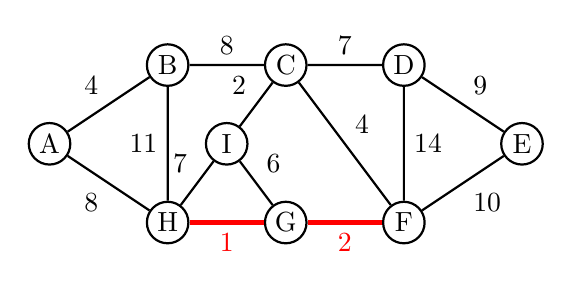
\begin{tikzpicture}[node distance={15mm}, thick, main/.style = {draw, circle}]
  \tikzstyle{vertex}=[circle,draw=black,thick,fill=white,minimum size=15pt, inner sep=0pt]
  \node[vertex] (A) at (0, 0) {A};
  \node[vertex] (B) at (1.5, 1) {B};
  \node[vertex] (C) at (3, 1) {C};
  \node[vertex] (D) at (4.5, 1) {D};
  \node[vertex] (E) at (6, 0) {E};
  \node[vertex] (F) at (4.5, -1) {F};
  \node[vertex] (G) at (3, -1) {G};
  \node[vertex] (H) at (1.5, -1) {H};
  \node[vertex] (I) at (2.25, 0) {I};
  \draw
  (A) -- node[anchor=south east]{4} (B)
  (B) -- node[above]{8} (C)
  (C) -- node[above]{7} (D)
  (D) -- node[anchor=south west]{9} (E)
  (E) -- node[anchor=north west]{10} (F)
  (A) -- node[anchor=north east]{8} (H)
  (B) -- node[left]{11} (H)
  (D) -- node[right]{14} (F)
  (H) -- node[anchor=south east]{7} (I)
  (C) -- node[anchor=south west]{4} (F)
  (I) -- node[anchor=south west]{6} (G)
  (I) -- node[anchor=south east]{2} (C)
  ;
  \draw[ultra thick,red]
  (G) -- node[below]{1} (H)
  (F) -- node[below]{2} (G)
  ;
\end{tikzpicture}

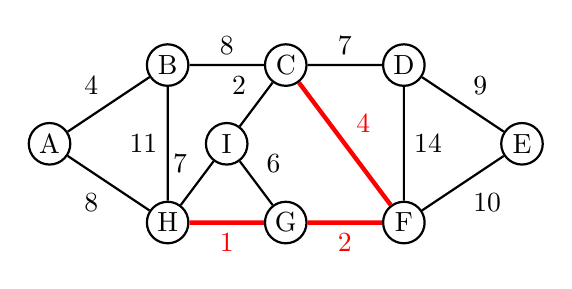
\begin{tikzpicture}[node distance={15mm}, thick, main/.style = {draw, circle}]
  \tikzstyle{vertex}=[circle,draw=black,thick,fill=white,minimum size=15pt, inner sep=0pt]
  \node[vertex] (A) at (0, 0) {A};
  \node[vertex] (B) at (1.5, 1) {B};
  \node[vertex] (C) at (3, 1) {C};
  \node[vertex] (D) at (4.5, 1) {D};
  \node[vertex] (E) at (6, 0) {E};
  \node[vertex] (F) at (4.5, -1) {F};
  \node[vertex] (G) at (3, -1) {G};
  \node[vertex] (H) at (1.5, -1) {H};
  \node[vertex] (I) at (2.25, 0) {I};
  \draw
  (A) -- node[anchor=south east]{4} (B)
  (B) -- node[above]{8} (C)
  (C) -- node[above]{7} (D)
  (D) -- node[anchor=south west]{9} (E)
  (E) -- node[anchor=north west]{10} (F)
  (A) -- node[anchor=north east]{8} (H)
  (B) -- node[left]{11} (H)
  (D) -- node[right]{14} (F)
  (H) -- node[anchor=south east]{7} (I)
  (I) -- node[anchor=south west]{6} (G)
  (I) -- node[anchor=south east]{2} (C)
  ;
  \draw[ultra thick,red]
  (G) -- node[below]{1} (H)
  (F) -- node[below]{2} (G)
  (C) -- node[anchor=south west]{4} (F)
  ;
\end{tikzpicture}
\quad\quad
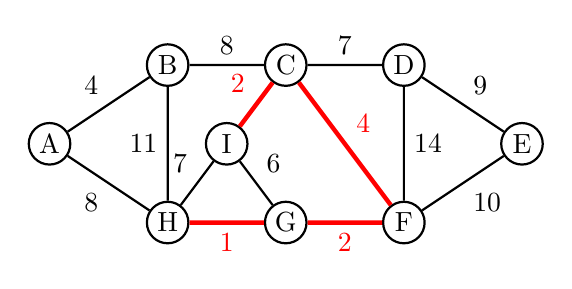
\begin{tikzpicture}[node distance={15mm}, thick, main/.style = {draw, circle}]
  \tikzstyle{vertex}=[circle,draw=black,thick,fill=white,minimum size=15pt, inner sep=0pt]
  \node[vertex] (A) at (0, 0) {A};
  \node[vertex] (B) at (1.5, 1) {B};
  \node[vertex] (C) at (3, 1) {C};
  \node[vertex] (D) at (4.5, 1) {D};
  \node[vertex] (E) at (6, 0) {E};
  \node[vertex] (F) at (4.5, -1) {F};
  \node[vertex] (G) at (3, -1) {G};
  \node[vertex] (H) at (1.5, -1) {H};
  \node[vertex] (I) at (2.25, 0) {I};
  \draw
  (A) -- node[anchor=south east]{4} (B)
  (B) -- node[above]{8} (C)
  (C) -- node[above]{7} (D)
  (D) -- node[anchor=south west]{9} (E)
  (E) -- node[anchor=north west]{10} (F)
  (A) -- node[anchor=north east]{8} (H)
  (B) -- node[left]{11} (H)
  (D) -- node[right]{14} (F)
  (H) -- node[anchor=south east]{7} (I)
  (I) -- node[anchor=south west]{6} (G)
  ;
  \draw[ultra thick,red]
  (G) -- node[below]{1} (H)
  (F) -- node[below]{2} (G)
  (C) -- node[anchor=south west]{4} (F)
  (I) -- node[anchor=south east]{2} (C)
  ;
\end{tikzpicture}

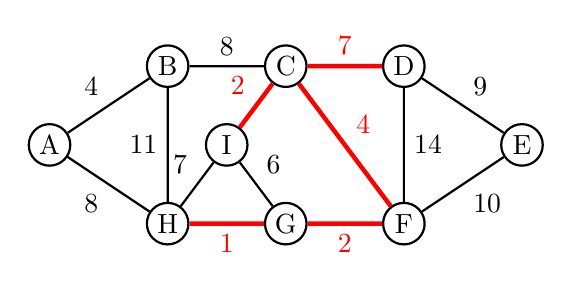
\begin{tikzpicture}[node distance={15mm}, thick, main/.style = {draw, circle}]
  \tikzstyle{vertex}=[circle,draw=black,thick,fill=white,minimum size=15pt, inner sep=0pt]
  \node[vertex] (A) at (0, 0) {A};
  \node[vertex] (B) at (1.5, 1) {B};
  \node[vertex] (C) at (3, 1) {C};
  \node[vertex] (D) at (4.5, 1) {D};
  \node[vertex] (E) at (6, 0) {E};
  \node[vertex] (F) at (4.5, -1) {F};
  \node[vertex] (G) at (3, -1) {G};
  \node[vertex] (H) at (1.5, -1) {H};
  \node[vertex] (I) at (2.25, 0) {I};
  \draw
  (A) -- node[anchor=south east]{4} (B)
  (B) -- node[above]{8} (C)
  (D) -- node[anchor=south west]{9} (E)
  (E) -- node[anchor=north west]{10} (F)
  (A) -- node[anchor=north east]{8} (H)
  (B) -- node[left]{11} (H)
  (D) -- node[right]{14} (F)
  (H) -- node[anchor=south east]{7} (I)
  (I) -- node[anchor=south west]{6} (G)
  ;
  \draw[ultra thick,red]
  (G) -- node[below]{1} (H)
  (F) -- node[below]{2} (G)
  (C) -- node[anchor=south west]{4} (F)
  (I) -- node[anchor=south east]{2} (C)
  (C) -- node[above]{7} (D)
  ;
\end{tikzpicture}
\quad\quad
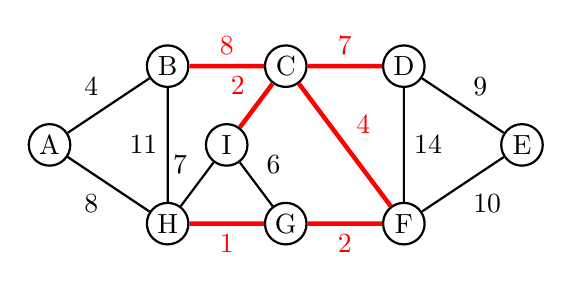
\begin{tikzpicture}[node distance={15mm}, thick, main/.style = {draw, circle}]
  \tikzstyle{vertex}=[circle,draw=black,thick,fill=white,minimum size=15pt, inner sep=0pt]
  \node[vertex] (A) at (0, 0) {A};
  \node[vertex] (B) at (1.5, 1) {B};
  \node[vertex] (C) at (3, 1) {C};
  \node[vertex] (D) at (4.5, 1) {D};
  \node[vertex] (E) at (6, 0) {E};
  \node[vertex] (F) at (4.5, -1) {F};
  \node[vertex] (G) at (3, -1) {G};
  \node[vertex] (H) at (1.5, -1) {H};
  \node[vertex] (I) at (2.25, 0) {I};
  \draw
  (A) -- node[anchor=south east]{4} (B)
  (D) -- node[anchor=south west]{9} (E)
  (E) -- node[anchor=north west]{10} (F)
  (A) -- node[anchor=north east]{8} (H)
  (B) -- node[left]{11} (H)
  (D) -- node[right]{14} (F)
  (H) -- node[anchor=south east]{7} (I)
  (I) -- node[anchor=south west]{6} (G)
  ;
  \draw[ultra thick,red]
  (G) -- node[below]{1} (H)
  (F) -- node[below]{2} (G)
  (C) -- node[anchor=south west]{4} (F)
  (I) -- node[anchor=south east]{2} (C)
  (C) -- node[above]{7} (D)
  (B) -- node[above]{8} (C)
  ;
\end{tikzpicture}

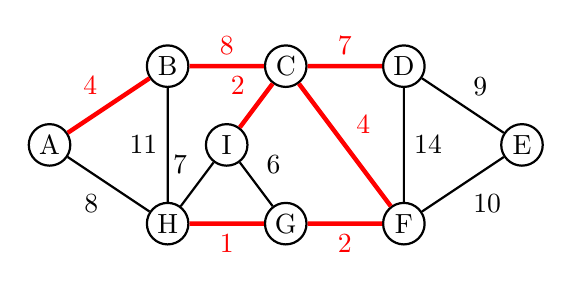
\begin{tikzpicture}[node distance={15mm}, thick, main/.style = {draw, circle}]
  \tikzstyle{vertex}=[circle,draw=black,thick,fill=white,minimum size=15pt, inner sep=0pt]
  \node[vertex] (A) at (0, 0) {A};
  \node[vertex] (B) at (1.5, 1) {B};
  \node[vertex] (C) at (3, 1) {C};
  \node[vertex] (D) at (4.5, 1) {D};
  \node[vertex] (E) at (6, 0) {E};
  \node[vertex] (F) at (4.5, -1) {F};
  \node[vertex] (G) at (3, -1) {G};
  \node[vertex] (H) at (1.5, -1) {H};
  \node[vertex] (I) at (2.25, 0) {I};
  \draw
  (D) -- node[anchor=south west]{9} (E)
  (E) -- node[anchor=north west]{10} (F)
  (A) -- node[anchor=north east]{8} (H)
  (B) -- node[left]{11} (H)
  (D) -- node[right]{14} (F)
  (H) -- node[anchor=south east]{7} (I)
  (I) -- node[anchor=south west]{6} (G)
  ;
  \draw[ultra thick,red]
  (G) -- node[below]{1} (H)
  (F) -- node[below]{2} (G)
  (C) -- node[anchor=south west]{4} (F)
  (I) -- node[anchor=south east]{2} (C)
  (C) -- node[above]{7} (D)
  (B) -- node[above]{8} (C)
  (A) -- node[anchor=south east]{4} (B)
  ;
\end{tikzpicture}
\quad\quad
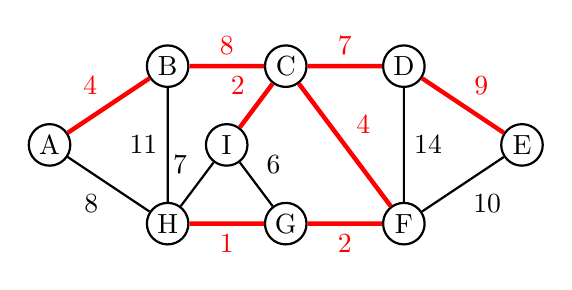
\begin{tikzpicture}[node distance={15mm}, thick, main/.style = {draw, circle}]
  \tikzstyle{vertex}=[circle,draw=black,thick,fill=white,minimum size=15pt, inner sep=0pt]
  \node[vertex] (A) at (0, 0) {A};
  \node[vertex] (B) at (1.5, 1) {B};
  \node[vertex] (C) at (3, 1) {C};
  \node[vertex] (D) at (4.5, 1) {D};
  \node[vertex] (E) at (6, 0) {E};
  \node[vertex] (F) at (4.5, -1) {F};
  \node[vertex] (G) at (3, -1) {G};
  \node[vertex] (H) at (1.5, -1) {H};
  \node[vertex] (I) at (2.25, 0) {I};
  \draw
  (E) -- node[anchor=north west]{10} (F)
  (A) -- node[anchor=north east]{8} (H)
  (B) -- node[left]{11} (H)
  (D) -- node[right]{14} (F)
  (H) -- node[anchor=south east]{7} (I)
  (I) -- node[anchor=south west]{6} (G)
  ;
  \draw[ultra thick,red]
  (G) -- node[below]{1} (H)
  (F) -- node[below]{2} (G)
  (C) -- node[anchor=south west]{4} (F)
  (I) -- node[anchor=south east]{2} (C)
  (C) -- node[above]{7} (D)
  (B) -- node[above]{8} (C)
  (A) -- node[anchor=south east]{4} (B)
  (D) -- node[anchor=south west]{9} (E)
  ;
\end{tikzpicture}

\textbf{Kruskal's Algorithm}

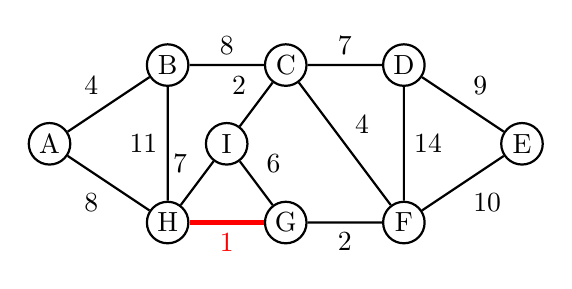
\begin{tikzpicture}[node distance={15mm}, thick, main/.style = {draw, circle}]
  \tikzstyle{vertex}=[circle,draw=black,thick,fill=white,minimum size=15pt, inner sep=0pt]
  \node[vertex] (A) at (0, 0) {A};
  \node[vertex] (B) at (1.5, 1) {B};
  \node[vertex] (C) at (3, 1) {C};
  \node[vertex] (D) at (4.5, 1) {D};
  \node[vertex] (E) at (6, 0) {E};
  \node[vertex] (F) at (4.5, -1) {F};
  \node[vertex] (G) at (3, -1) {G};
  \node[vertex] (H) at (1.5, -1) {H};
  \node[vertex] (I) at (2.25, 0) {I};
  \draw
  (A) -- node[anchor=south east]{4} (B)
  (B) -- node[above]{8} (C)
  (C) -- node[above]{7} (D)
  (D) -- node[anchor=south west]{9} (E)
  (E) -- node[anchor=north west]{10} (F)
  (F) -- node[below]{2} (G)
  (A) -- node[anchor=north east]{8} (H)
  (B) -- node[left]{11} (H)
  (D) -- node[right]{14} (F)
  (H) -- node[anchor=south east]{7} (I)
  (C) -- node[anchor=south west]{4} (F)
  (I) -- node[anchor=south west]{6} (G)
  (I) -- node[anchor=south east]{2} (C)
  ;
  \draw[ultra thick,red]
  (G) -- node[below]{1} (H)
  ;
\end{tikzpicture}
\quad\quad
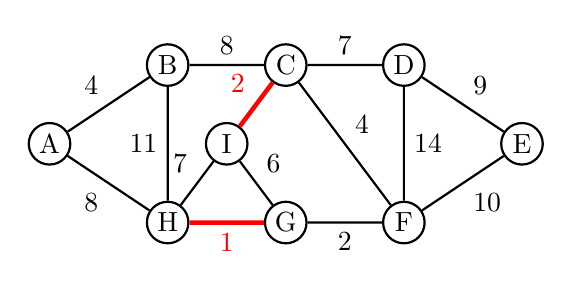
\begin{tikzpicture}[node distance={15mm}, thick, main/.style = {draw, circle}]
  \tikzstyle{vertex}=[circle,draw=black,thick,fill=white,minimum size=15pt, inner sep=0pt]
  \node[vertex] (A) at (0, 0) {A};
  \node[vertex] (B) at (1.5, 1) {B};
  \node[vertex] (C) at (3, 1) {C};
  \node[vertex] (D) at (4.5, 1) {D};
  \node[vertex] (E) at (6, 0) {E};
  \node[vertex] (F) at (4.5, -1) {F};
  \node[vertex] (G) at (3, -1) {G};
  \node[vertex] (H) at (1.5, -1) {H};
  \node[vertex] (I) at (2.25, 0) {I};
  \draw
  (A) -- node[anchor=south east]{4} (B)
  (B) -- node[above]{8} (C)
  (C) -- node[above]{7} (D)
  (D) -- node[anchor=south west]{9} (E)
  (E) -- node[anchor=north west]{10} (F)
  (F) -- node[below]{2} (G)
  (A) -- node[anchor=north east]{8} (H)
  (B) -- node[left]{11} (H)
  (D) -- node[right]{14} (F)
  (H) -- node[anchor=south east]{7} (I)
  (C) -- node[anchor=south west]{4} (F)
  (I) -- node[anchor=south west]{6} (G)
  ;
  \draw[ultra thick,red]
  (G) -- node[below]{1} (H)
  (I) -- node[anchor=south east]{2} (C)
  ;
\end{tikzpicture}

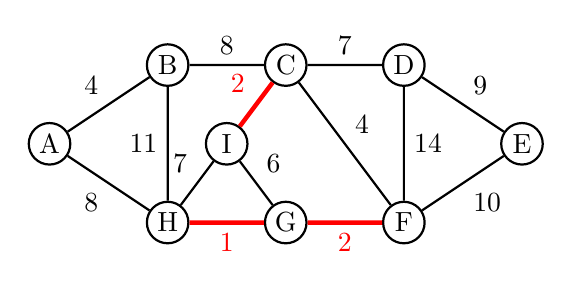
\begin{tikzpicture}[node distance={15mm}, thick, main/.style = {draw, circle}]
  \tikzstyle{vertex}=[circle,draw=black,thick,fill=white,minimum size=15pt, inner sep=0pt]
  \node[vertex] (A) at (0, 0) {A};
  \node[vertex] (B) at (1.5, 1) {B};
  \node[vertex] (C) at (3, 1) {C};
  \node[vertex] (D) at (4.5, 1) {D};
  \node[vertex] (E) at (6, 0) {E};
  \node[vertex] (F) at (4.5, -1) {F};
  \node[vertex] (G) at (3, -1) {G};
  \node[vertex] (H) at (1.5, -1) {H};
  \node[vertex] (I) at (2.25, 0) {I};
  \draw
  (A) -- node[anchor=south east]{4} (B)
  (B) -- node[above]{8} (C)
  (C) -- node[above]{7} (D)
  (D) -- node[anchor=south west]{9} (E)
  (E) -- node[anchor=north west]{10} (F)
  (A) -- node[anchor=north east]{8} (H)
  (B) -- node[left]{11} (H)
  (D) -- node[right]{14} (F)
  (H) -- node[anchor=south east]{7} (I)
  (C) -- node[anchor=south west]{4} (F)
  (I) -- node[anchor=south west]{6} (G)
  ;
  \draw[ultra thick,red]
  (G) -- node[below]{1} (H)
  (I) -- node[anchor=south east]{2} (C)
  (F) -- node[below]{2} (G)
  ;
\end{tikzpicture}
\quad\quad
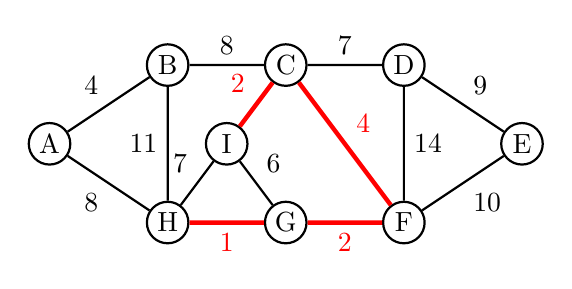
\begin{tikzpicture}[node distance={15mm}, thick, main/.style = {draw, circle}]
  \tikzstyle{vertex}=[circle,draw=black,thick,fill=white,minimum size=15pt, inner sep=0pt]
  \node[vertex] (A) at (0, 0) {A};
  \node[vertex] (B) at (1.5, 1) {B};
  \node[vertex] (C) at (3, 1) {C};
  \node[vertex] (D) at (4.5, 1) {D};
  \node[vertex] (E) at (6, 0) {E};
  \node[vertex] (F) at (4.5, -1) {F};
  \node[vertex] (G) at (3, -1) {G};
  \node[vertex] (H) at (1.5, -1) {H};
  \node[vertex] (I) at (2.25, 0) {I};
  \draw
  (A) -- node[anchor=south east]{4} (B)
  (B) -- node[above]{8} (C)
  (C) -- node[above]{7} (D)
  (D) -- node[anchor=south west]{9} (E)
  (E) -- node[anchor=north west]{10} (F)
  (A) -- node[anchor=north east]{8} (H)
  (B) -- node[left]{11} (H)
  (D) -- node[right]{14} (F)
  (H) -- node[anchor=south east]{7} (I)
  (I) -- node[anchor=south west]{6} (G)
  ;
  \draw[ultra thick,red]
  (G) -- node[below]{1} (H)
  (I) -- node[anchor=south east]{2} (C)
  (F) -- node[below]{2} (G)
  (C) -- node[anchor=south west]{4} (F)
  ;
\end{tikzpicture}

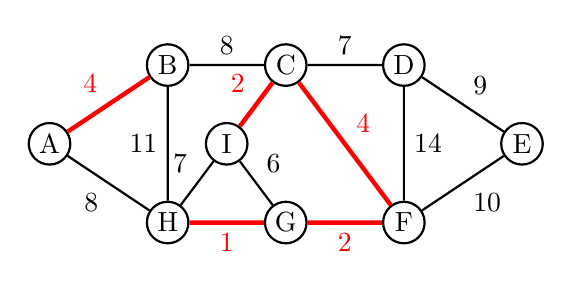
\begin{tikzpicture}[node distance={15mm}, thick, main/.style = {draw, circle}]
  \tikzstyle{vertex}=[circle,draw=black,thick,fill=white,minimum size=15pt, inner sep=0pt]
  \node[vertex] (A) at (0, 0) {A};
  \node[vertex] (B) at (1.5, 1) {B};
  \node[vertex] (C) at (3, 1) {C};
  \node[vertex] (D) at (4.5, 1) {D};
  \node[vertex] (E) at (6, 0) {E};
  \node[vertex] (F) at (4.5, -1) {F};
  \node[vertex] (G) at (3, -1) {G};
  \node[vertex] (H) at (1.5, -1) {H};
  \node[vertex] (I) at (2.25, 0) {I};
  \draw
  (B) -- node[above]{8} (C)
  (C) -- node[above]{7} (D)
  (D) -- node[anchor=south west]{9} (E)
  (E) -- node[anchor=north west]{10} (F)
  (A) -- node[anchor=north east]{8} (H)
  (B) -- node[left]{11} (H)
  (D) -- node[right]{14} (F)
  (H) -- node[anchor=south east]{7} (I)
  (I) -- node[anchor=south west]{6} (G)
  ;
  \draw[ultra thick,red]
  (G) -- node[below]{1} (H)
  (I) -- node[anchor=south east]{2} (C)
  (F) -- node[below]{2} (G)
  (C) -- node[anchor=south west]{4} (F)
  (A) -- node[anchor=south east]{4} (B)
  ;
\end{tikzpicture}
\quad\quad
\begin{tikzpicture}[node distance={15mm}, thick, main/.style = {draw, circle}]
  \tikzstyle{vertex}=[circle,draw=black,thick,fill=white,minimum size=15pt, inner sep=0pt]
  \node[vertex] (A) at (0, 0) {A};
  \node[vertex] (B) at (1.5, 1) {B};
  \node[vertex] (C) at (3, 1) {C};
  \node[vertex] (D) at (4.5, 1) {D};
  \node[vertex] (E) at (6, 0) {E};
  \node[vertex] (F) at (4.5, -1) {F};
  \node[vertex] (G) at (3, -1) {G};
  \node[vertex] (H) at (1.5, -1) {H};
  \node[vertex] (I) at (2.25, 0) {I};
  \draw
  (B) -- node[above]{8} (C)
  (D) -- node[anchor=south west]{9} (E)
  (E) -- node[anchor=north west]{10} (F)
  (A) -- node[anchor=north east]{8} (H)
  (B) -- node[left]{11} (H)
  (D) -- node[right]{14} (F)
  (H) -- node[anchor=south east]{7} (I)
  (I) -- node[anchor=south west]{6} (G)
  ;
  \draw[ultra thick,red]
  (G) -- node[below]{1} (H)
  (I) -- node[anchor=south east]{2} (C)
  (F) -- node[below]{2} (G)
  (C) -- node[anchor=south west]{4} (F)
  (A) -- node[anchor=south east]{4} (B)
  (C) -- node[above]{7} (D)
  ;
\end{tikzpicture}

\begin{tikzpicture}[node distance={15mm}, thick, main/.style = {draw, circle}]
  \tikzstyle{vertex}=[circle,draw=black,thick,fill=white,minimum size=15pt, inner sep=0pt]
  \node[vertex] (A) at (0, 0) {A};
  \node[vertex] (B) at (1.5, 1) {B};
  \node[vertex] (C) at (3, 1) {C};
  \node[vertex] (D) at (4.5, 1) {D};
  \node[vertex] (E) at (6, 0) {E};
  \node[vertex] (F) at (4.5, -1) {F};
  \node[vertex] (G) at (3, -1) {G};
  \node[vertex] (H) at (1.5, -1) {H};
  \node[vertex] (I) at (2.25, 0) {I};
  \draw
  (B) -- node[above]{8} (C)
  (D) -- node[anchor=south west]{9} (E)
  (E) -- node[anchor=north west]{10} (F)
  (B) -- node[left]{11} (H)
  (D) -- node[right]{14} (F)
  (I) -- node[anchor=south west]{6} (G)
  (H) -- node[anchor=south east]{7} (I)
  ;
  \draw[ultra thick,red]
  (G) -- node[below]{1} (H)
  (I) -- node[anchor=south east]{2} (C)
  (F) -- node[below]{2} (G)
  (C) -- node[anchor=south west]{4} (F)
  (A) -- node[anchor=south east]{4} (B)
  (C) -- node[above]{7} (D)
  (A) -- node[anchor=north east]{8} (H)
  ;
\end{tikzpicture}
\quad\quad
\begin{tikzpicture}[node distance={15mm}, thick, main/.style = {draw, circle}]
  \tikzstyle{vertex}=[circle,draw=black,thick,fill=white,minimum size=15pt, inner sep=0pt]
  \node[vertex] (A) at (0, 0) {A};
  \node[vertex] (B) at (1.5, 1) {B};
  \node[vertex] (C) at (3, 1) {C};
  \node[vertex] (D) at (4.5, 1) {D};
  \node[vertex] (E) at (6, 0) {E};
  \node[vertex] (F) at (4.5, -1) {F};
  \node[vertex] (G) at (3, -1) {G};
  \node[vertex] (H) at (1.5, -1) {H};
  \node[vertex] (I) at (2.25, 0) {I};
  \draw
  (B) -- node[above]{8} (C)
  (E) -- node[anchor=north west]{10} (F)
  (B) -- node[left]{11} (H)
  (D) -- node[right]{14} (F)
  (I) -- node[anchor=south west]{6} (G)
  (H) -- node[anchor=south east]{7} (I)
  ;
  \draw[ultra thick,red]
  (G) -- node[below]{1} (H)
  (I) -- node[anchor=south east]{2} (C)
  (F) -- node[below]{2} (G)
  (C) -- node[anchor=south west]{4} (F)
  (A) -- node[anchor=south east]{4} (B)
  (C) -- node[above]{7} (D)
  (A) -- node[anchor=north east]{8} (H)
  (D) -- node[anchor=south west]{9} (E)
  ;
\end{tikzpicture}
\end{eg}

% END OF DOCUMENT